\section{HW3}
For each of the sentences below give an LF and derive the semantics of the sentence from this LF in the way we have been doing for the exercises on the 3d practice homework (that is, by assigning Lambda Calculus terms to the nodes of the LF tree).

In (2) and (5) only choose an LF for what you take to be the most plausible scope ordering.
\begin{QandA}
   \item Pedro owns a donkey. 
         \begin{answered}
			\begin{tikzpicture}[scale=1]
			\tikzset{level 1+/.style={level distance=30pt}}
			\tikzset{every tree node/.style={align=left,anchor=north}}
			\Tree [.S
			  [.DP Pedrow ]
			  [.VP
			    [.$V_{tr}$ owns ]
			    [.DP
			      [.Det a ]
			      [.NP donkey ] 
			    ]  
			  ] 
			]
         	\end{tikzpicture}
         	
			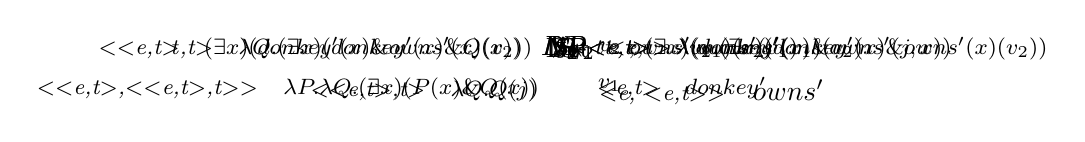
\begin{tikzpicture}[scale=0.7]
			\tikzset{level 1+/.style={level distance=30pt}}
			\tikzset{every tree node/.style={align=left,anchor=north}}
			\Tree [. \node[label={right:{\textit{\footnotesize t \space;\space $(\exists x)(donkey'(x) \& owns'(j,x))$}}}]{$S \star$};
			  [. \node[label={below left:\textit{ \footnotesize $<<$e,t$>$,t$>$ \space\space $\lambda Q. Q(j)$}}]{$DP_2$}; Pedro ]
			     [.\node[label={right:\textit{\footnotesize $<$e,t$>$ \space\space $\lambda v_2. (\exists x)(donkey'(x) \& owns'(x)(v_2))$}}]{}; 
			       [.2 ] 
			       [.\node[label={left:\textit{\footnotesize t \space\space $(\exists x)(donkey'(x) \& owns'(x)(v_2))$}}]{$S \ast$};
			         [.\node[label={left:\textit{\footnotesize $<<$e,t$>$,t$>$ \space\space $\lambda Q. (\exists x)(donkey'(x) \& Q(x))$}}]{$DP_1$}; 
			           [.\node[label={below left:\textit{\footnotesize $<<$e,t$>$,$<<$e,t$>$,t$>>$ \space\space $\lambda P. \lambda Q. (\exists x)(P(x) \& Q(x))$ }}]{Det}; a ]
			           [.\node[label={below right:\textit{\footnotesize $<$e,t$>$ \space\space $donkey'$}}]{NP}; donkey ]
			         ]
			         [.\node[label={right:\textit{\footnotesize $<$e,t$>$ \space\space $\lambda v_1 . owns'(v_1)(v_2)$}}]{};
			           [.1 ]
			           [.\node[label={right:\textit{\footnotesize $t$ \space\space $owns'(v_1)(v_2)$}}]{S};
			             [.\node[label={right:\textit{\footnotesize $v_2$ }}]{$t_2$};]
			             [.\node[label={right:\textit{\footnotesize $<$e,t$>$ \space\space $owns'(v_1)$ }}]{VP};
			               [.\node[label={below right:\textit{\footnotesize $<$e, $<$e,t$>$$>$} \space\space $owns'$}]{$V_{tr}$}; owns ]
			               [.\node[label={below right:\textit{\footnotesize $v_1$ }}]{$t_1$};]
			             ]
			           ]
			         ]
			       ]
			     ]
			  ]
			\end{tikzpicture}
 		 \begin{align*}
 		 \ast & =\lambda Q. (\exists x)(donkey'(x) \& Q(x))(\lambda v_1 owns'(v_1)(v_2)) \\
 		 & = (\exists x)(donkey'(x) \& (\lambda v_1 owns'(v_1)(v_2))(x)) \\
 		 & = (\exists x)(donkey'(x) \& owns'(x)(v_2)) \\ \\
 		 \star & =(\lambda Q. Q(j))(\lambda v_2. (\exists x)(donkey'(x) \& owns'(x)(v_2))) \\
 		 & = (\lambda v_2.(\exists x)(donkey'(x) \& owns'(x)(v_2)))(j) \\
 		 & = (\exists x)(donkey'(x) \& owns'(x)(j)) \\
 		 & = (\exists x)(donkey'(x) \& owns'(j,x))
 		 \end{align*}

         \end{answered}

   \item Somebody likes nobody.
         \begin{tikzpicture}[scale=1]
   			\tikzset{level 1+/.style={level distance=30pt}}
   			\tikzset{every tree node/.style={align=left,anchor=north}}
   			\Tree [.S
   			  [.DP Somebody ]
   			  [.VP
   			    [.$V_{tr}$ likes ]
   			    [.DP nobody ]  
   			  ] 
   			]
         \end{tikzpicture}
   
         \begin{answered}
			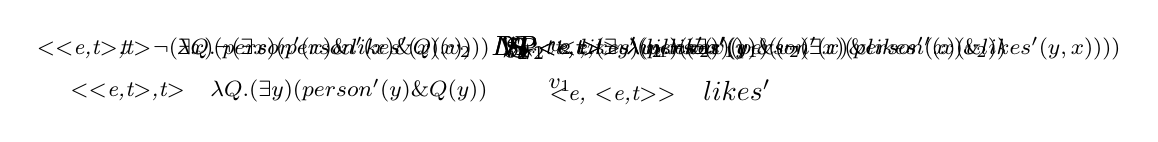
\begin{tikzpicture}[scale=0.75]
			\tikzset{level 1+/.style={level distance=30pt}}
			\tikzset{every tree node/.style={align=left,anchor=north}}
			\Tree [. \node[label={right:{\textit{\footnotesize t \space;\space $(\exists y)(person'(y) \& (\neg (\exists x)(person'(x) \& likes'(y,x))))$}}}]{$S \star$};
			  [. \node[label={below left:\textit{ \footnotesize $<<$e,t$>$,t$>$ \space\space $\lambda Q. (\exists y)(person'(y) \& Q(y))$}}]{$DP_2$}; Somebody ]
			     [.\node[label={right:\textit{\footnotesize $<$e,t$>$ \space\space $\lambda v_2. \neg (\exists x)(person'(x) \& likes'(x)(v_2))$}}]{}; 
			       [.2 ] 
			       [.\node[label={left:\textit{\footnotesize t \space\space $\neg (\exists x)(person'(x) \& likes'(x)(v_2))$}}]{$S$};
			         [.\node[label={left:\textit{\footnotesize $<<$e,t$>$,t$>$ \space\space $\lambda Q. \neg (\exists x)(person'(x) \& Q(x))$}}]{$DP_1$}; nobody ]
			         [.\node[label={right:\textit{\footnotesize $<$e,t$>$ \space\space $\lambda v_1 . likes'(v_1)(v_2)$}}]{};
			           [.1 ]
			           [.\node[label={right:\textit{\footnotesize $t$ \space\space $likes'(v_1)(v_2)$}}]{S};
			             [.\node[label={right:\textit{\footnotesize $v_2$ }}]{$t_2$};]
			             [.\node[label={right:\textit{\footnotesize $<$e,t$>$ \space\space $likes'(v_1)$ }}]{VP};
			               [.\node[label={below right:\textit{\footnotesize $<$e, $<$e,t$>$$>$} \space\space $likes'$}]{$V_{tr}$}; likes ]
			               [.\node[label={below right:\textit{\footnotesize $v_1$ }}]{$t_1$};]
			             ]
			           ]
			         ]
			       ]
			     ]
			  ]
			\end{tikzpicture}
			\begin{align*}
	 		 \star & =(\lambda Q. (\exists y)(person'(y) \& Q(y)))(\lambda v_2. \neg (\exists x)(person'(x) \& likes'(x)(v_2))) \\
	 		 & = (\exists y)(person'(y) \& (\lambda v_2. \neg (\exists x)(person'(x) \& likes'(x)(v_2))(y))) \\
	 		 & = (\exists y)(person'(y) \& (\neg (\exists x)(person'(x) \& likes'(x)(y)))) \\
	 		 & = (\exists y)(person'(y) \& (\neg (\exists x)(person'(x) \& likes'(y,x))))
			\end{align*}
         \end{answered}
         
   \item Every sensible person who likes Mozart likes Haydn.
         \begin{answered}
         \begin{tikzpicture}[scale=1]
   			\tikzset{level 1+/.style={level distance=30pt}}
   			\tikzset{every tree node/.style={align=left,anchor=north}}
   			\Tree [.S
   			  [.DP 
   			    [.Det every ]
   			    [.NP
   			      [.AP sensible ]
   			      [.NP
   			        [.NP person ]
   			        [.RC
   			          [.Comp who ]
   			          [.VP
   			            [.$V_{tr}$ likes ]
   			            [.DP Mozart ] 
   			          ]
   			        ] 
   			      ] 
   			    ]
   			  ]
   			  [.VP
   			    [.$V_{tr}$ likes ]
   			    [.DP Haydn ]  
   			  ] 
   			]
         \end{tikzpicture}
         
		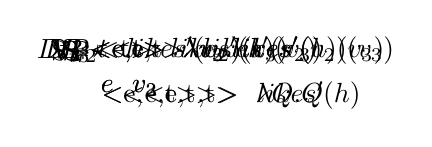
\begin{tikzpicture}[scale=0.8]
		\Tree [.\node {S $\ast$};
		        [.\node(site){$DP_3 \star$}; ]
		        [.\node [label={right: $<$e,t$>$ \space $\lambda v_3. likes'(h)(v_3)$}]{}; 
		          [.3 ]
		          [.\node [label={right: $<$t$>$ \space $likes'(h)(v_3)$}] {S};
		            [.\node [label={below right: $<<$e,t$>$,t$>$ \space $\lambda Q. Q(h)$}] {$DP_2$}; Hayden ]
		            [.\node [label={right: $<$e,t$>$ \space $\lambda v_2. likes'(v_2)(v_3)$}] {};
		              [.2 ]
		              [.\node [label={right: $t$ \space $likes'(v_2)(v_3)$}] {S}; 
		                [.\node [label={below right: $e$ \space $v_3$}] {$t_3$}; ]
		                [.\node [label={right: $<$e,t$>$ \space $likes'(v_2)$}] {VP};
		                  [.\node [label={below right: $<$e,$<$e,t$>>$ \space $likes'$}] {$V_{tr}$}; likes ]
		                  [.\node [label={below right: $e$ \space $v_2$}] {$t_2$}; ]
		                ]
		              ]
		            ]
		          ]
		        ]
		      ]
		\end{tikzpicture}
		
		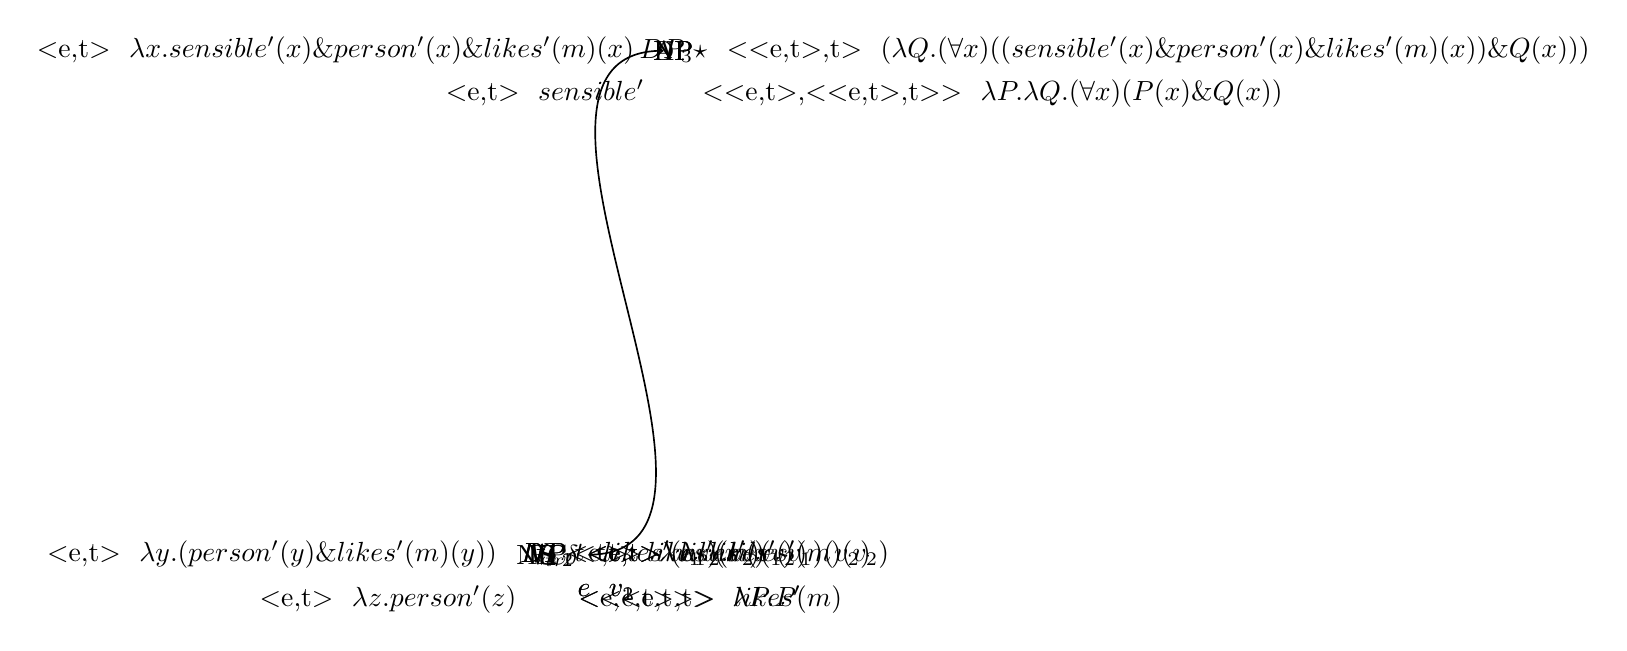
\begin{tikzpicture}[scale=0.8]
		\tikzset{level 1+/.style={level distance=30pt}}
		\tikzset{every tree node/.style={align=left,anchor=north}}
		\begin{scope}
		\Tree [.\node [label={right: $<<$e,t$>$,t$>$ \space $(\lambda Q. (\forall x)((sensible'(x) \& person'(x) \& likes'(m)(x)) \& Q(x)))$ }] {$DP_3 \star$}; 
		        [.\node [label={below right: $<<$e,t$>$,$<<$e,t$>$,t$>>$ \space $\lambda P. \lambda Q. (\forall x)(P(x) \& Q(x))$ }] {DP}; every ]
		        [.\node [label={left: $<$e,t$>$ \space $\lambda x. sensible'(x) \& person'(x) \& likes'(m)(x)$}] {NP};
		          [.\node(empty){~}; ]
		          [.\node [label={below left: $<$e,t$>$ \space $sensible'$}] {AP}; sensible ]
%		          [.\node [label={right: $<$e,t$>$ \space $\lambda y. (person'(y) \& likes'(m)(y))$}] {NP};
%		            [.\node [label={below right: $<$e,t$>$ \space $person'$}] {$NP_2$}; person ]
%		            [.\node [label={right: $<$e,t$>$ \space $\lambda v_2. likes'(m)(v_2)$}] {RC}; 
%		              [.COMP who ]
%		              [.\node [label={right: $<$t$>$ \space $likes'(m)(v_2)$}] {S};
%		                [.\node [label={below right: $<<$e,t$>$,t$>$ \space $\lambda P. P(m)$}] {$DP_1$}; Mozart ]
%		                [.\node(empty) [label={right: $<$e,t$>$ \space $\lambda v_1. likes'(v_1)(v_2)$}] {};
%		                  [.1 ]
%		                  [.\node [label={right: $t$ \space $likes'(v_1)(v_2)$}] {S};
%		                    [.\node [label={below right: $e$ \space $v_2$}] {$t_2$}; ]
%		                    [.\node [label={right: $<$e,t$>$ \space $likes'(v_1)$}] {VP};
%		                      [.\node [label={below right: $<$e,$<$e,t$>>$ \space $likes'$}] {$V_{tr}$}; likes ]
%		                      [.\node [label={below right: $e$ \space $v_1$}] {$t_1$}; ]
%		                    ]
%		                  ]
%		                ]
%		              ]
%		            ]
%		          ]
		        ]
		      ]
		\end{scope}
		\begin{scope}[shift=({-2cm, -8cm})]
		[.1 ]
        \Tree [.\node (root) [label={left: $<$e,t$>$ \space $\lambda y. (person'(y) \& likes'(m)(y))$}] {NP $\delta$};
        		            [.\node [label={below left: $<$e,t$>$ \space $\lambda z. person'(z)$}] {$DP_2$}; person ]
        		            [.\node [label={right: $<$e,t$>$ \space $\lambda v_2. likes'(m)(v_2)$}] {RC}; 
        		              [.COMP who ]
        		              [.\node [label={right: $<$t$>$ \space $likes'(m)(v_2)$}] {S};
        		                [.\node [label={below right: $<<$e,t$>$,t$>$ \space $\lambda P. P(m)$}] {$DP_1$}; Mozart ]
        		                [.\node [label={right: $<$e,t$>$ \space $\lambda v_1. likes'(v_1)(v_2)$}] {};
        		                  [.1 ]
        		                  [.\node [label={right: $t$ \space $likes'(v_1)(v_2)$}] {S};
        		                    [.\node [label={below right: $e$ \space $v_2$}] {$t_2$}; ]
        		                    [.\node [label={right: $<$e,t$>$ \space $likes'(v_1)$}] {VP};
        		                      [.\node [label={below right: $<$e,$<$e,t$>>$ \space $likes'$}] {$V_{tr}$}; likes ]
        		                      [.\node [label={below right: $e$ \space $v_1$}] {$t_1$}; ]
        		                    ]
        		                  ]
        		                ]
        		              ]
        		            ]
        		          ]
		\end{scope}
		\draw[semithick,->] (root) to [out=0, in=180] (empty);
		\end{tikzpicture}
		
		\begin{align*}
		\delta & = (\lambda P. \lambda Q. \lambda y. (P(y) \& Q(y)))(\lambda v_2. likes'(m)(v_2))(\lambda z. person'(z)) \\
		& = (\lambda Q. \lambda y. ((\lambda z. person'(z))(y) \& Q(y)))(\lambda v_2. likes'(m)(v_2)) \\
		& = (\lambda Q. \lambda y. (person'(y) \& Q(y)))(\lambda v_2. likes'(m)(v_2)) \\
		& = \lambda y. (person'(y) \& (\lambda v_2. likes'(m)(v_2))(y)) \\
		& = \lambda y. (person'(y) \& likes'(m)(y))
		\end{align*}
		\begin{align*}
 		\star & =\lambda P. \lambda Q. (\forall x)(P(x) \& Q(x)))(\lambda x. sensible'(x) \& person'(x) \& likes'(m)(x) \\
 		& =  \lambda Q. (\forall x)((\lambda x. sensible'(x) \& person'(x) \& likes'(m)(x))(x) \& Q(x))\\
 		& = \lambda Q. (\forall x)((sensible'(x) \& person'(x) \& likes'(m)(x)) \& Q(x)) \\
 		\end{align*}
 		\begin{align*}
 		\ast & =\lambda Q. (\forall x)((sensible'(x) \& person'(x) \& likes'(m)(x)) \& Q(x)))(\lambda v_3. likes'(h)(v_3)) \\
 		& =  (\forall x)(sensible'(x) \& person'(x) \& likes'(m)(x) \& likes'(h)(x))\\
		\end{align*}
         
         \end{answered}
   \item An American farmer talked to a Canadian farmer. (Treat ‘talk to’ as a transitive verb.)
         \begin{answered}
		 TBA
         \end{answered}
   \item Not everybody who likes somebody likes everybody. (N.B. In (5) treat ‘not everybody’ as an unanalyzed determiner with the semantics:
   $\lambda P. \lambda Q. \neg (\forall x)(P(x)\rightarrow Q(x))$)
         \begin{answered}
		 TBA
         \end{answered}
\end{QandA}